\chapter{Annotation}
\label{chap:annotation}

I begin this chapter with a discussion of the development and implementation of an annotation scheme that captures aspects of native-likeness and accuracy that are appropriate for content analysis. In the second half of this chapter, I examine inter-annotator agreement for the individual annotation features on a sample of the responses.

\section{Annotation scheme}
\label{sec:scheme}
The goal of the annotation is to provide information that would be useful for the automatic content assessment of NNS responses via comparison with NS responses.  
%A five-dimension annotation scheme was developed to capture different facets of assessment.
%
%; insights gained from the annotation, and in particular an interannotator agreement study, are covered in section~\ref{sec:agreement}.
%
The annotation scheme was developed through an iterative process of annotation, discussion and revision, with input from two annotators and other language professionals. The annotation was applied to both NS and NNS responses. To avoid any potential bias, annotators received the responses in random order and without any demographic information. For NS responses, the annotation allows for weighting or filtering of a set of gold standard (GS) responses, which can be used to evaluate the NNS responses. The annotation also allows for evaluation of the appropriateness of crowdsourcing a GS for content assessment. For NNS responses, the annotation serves as a score which can be compared to scores provided by an automatic system, allowing for evaluation of the system itself. Furthermore, the annotation lends insights into which aspects of a response are the most difficult to account for in the current approach to content assessment.

The scheme was initially planned as a single three-point scale, ranging from \textit{accurate and native-like} to \textit{accurate but not native-like} to \textit{not accurate}. This proved problematic, however, as \textit{accuracy} and \textit{native-likeness} could not be adequately defined and applied to the data as a single score.
For example, in Table~\ref{fig:sample-responses}, it is not clear how native-like \textit{She is happy with the dog} is.  Grammatically, it is native-like, but it does not seem like an appropriate answer to the question, \textit{What is the woman doing?} Moreover, \textit{The dog is so happy!} may be native-like in terms of language use, but does not seem appropriate in the context of the question. Thus, for the purpose of analyzing content in PDT responses, native-likeness seems to encompass considerations beyond language use and grammar. 

Likewise, accuracy could not be satisfactorily defined as a simple \textit{yes} or \textit{no} construct. To illustrate, consider the ramifications of the response \textit{hugging her dog Fluffy that she missed while on vacation} (Table~\ref{fig:sample-responses}) as either a NS or NNS response. The response does capture the main action of the item, but embellishes with unknowable details like the dog's name and the subject's motivation. This kind of response is undesirable in its own right, but could also lead to real problems during the automatic scoring. If included in a gold standard (GS) set of NS responses which serve as the basis for scoring new NNS responses, this kind of embellishment would dilute the most salient and desirable information in the GS. Furthermore, if such a NNS response is annotated as accurate, this additional information is unlikely to be readily mapped to information found in the GS, which would lead to lower scores for the response. Accuracy, it seems, is an inadequate construct for the approach to content assessment envisioned for this work. Clearly, verifiability is an important consideration as well.

\begin{figure}[htb!]
%\begin{table}[t!] This line is giving me trouble when I go to typeset
\begin{center}
\begin{tabular}{|l|}
\hline
\multicolumn{1}{|c|}{
\includegraphics[width=0.45\columnwidth]{figures/I29.jpg}} \\
\hline
1. Holding a puppy and looks happy \\
\hline
2. She is happy with the dog. \\
\hline
3. She is wear a blue dress. \\
%3. The lady loves her dog. \\
\hline
4. hugging her dog Fluffy that she missed while on vacation. \\
\hline
5. The dog is so happy! \\
\hline
6. She loves her pet \\
\hline
\end{tabular}
\caption{\label{fig:sample-responses} Sample responses for the targeted item, \textit{What is the woman doing?}}
\end{center}
\end{figure}

In order to handle the kinds of meaningful variation observed in the responses, five binary features were eventually settled on, with each feature having some relation to the original concepts of accuracy and native-likeness. As with most annotation schemes, the final SAILS scheme is a compromise. This scheme represents the minimal set of features that I believe necessary to accomplish two major goals of this work: investigating the use of NS responses as a GS, and examining the factors that lead a NNS response to be rated highly or lowly. Besides the features explained below, others were explored but rejected. For example, a \textit{good faith} feature was considered to identify responses that were not given in good faith, such as gibberish, profanity and irrelevant responses. Such a discrimination was applicable to less than three percent of responses in the development set, however, so this feature was deemed too costly for the value it would provide.

A set of annotation guidelines were produced with definitions, rules and examples for each feature. For most features, the rules for targeted and untargeted items vary slightly; the untargeted rules are generally less strict to accommodate the less restrictive prompt question. The complete annotation guide is included in Appendix XYZ.\lk{xyz} The features and brief descriptions are listed here and discussed further in the discussion of inter-annotator agreement in Section~\ref{sec:agreement}.

\begin{enumerate}
\item \textbf{Core Event}: Does the response capture the core event depicted in the image? Core events are not pre-defined for annotators but should be clear given the stripped down nature of the images. Crucially, the response should link an appropriate subject to the event.  In Table~\ref{fig:sample-responses}, \textit{[The woman is] holding a puppy and looks happy} clearly captures the core event, while \textit{She is wear a blue dress} is irrelevant to the event happening.
\item \textbf{Verifiability}: Does the response contain only information that is true and verifiable based on the image? Inferences should not be speculations and are allowed only when necessary and highly probable, as when describing a familial or professional relationship between persons depicted in the image.  For example, in Table~\ref{fig:sample-responses}, \textit{She is wear a blue dress} conveys information that is irrelevant to the core event but is nonetheless recoverable from the image (core event=0, verifiability=1), while \textit{hugging her dog Fluffy that she missed while on vacation} fulfills the core event but also has information that cannot be inferred from the picture (core event=1, verifiability=0).
\item \textbf{Answerhood}: Does the response make a clear attempt to answer the prompt question? This generally requires a progressive verb. For targeted items, the subject of the question or an appropriate pronoun must be used as the subject of the response.  For example, \textit{The dog is so happy!} is answering a question other than \textit{What is the woman doing?}. 
\item \textbf{Interpretability}: Does the response evoke a clear mental image (even if different from the actual item image)? Any required verb arguments must be present and unambiguous.  For example, \textit{She loves her pet} is too vague to generate a clear mental image. No action is specified (unless we force an unlikely reading of \textit{loves} as a dynamic, simple present verb), and we cannot know if the \textit{pet} is a dog, a horse, etc.
\item \textbf{Grammaticality}: Is the response free from errors of spelling and grammar?  
%While the focus of GEC work, 
This is a relatively straightforward feature to annotate. For example, from Table~\ref{fig:sample-responses}, \textit{She is wear a blue dress} contains an ungrammatical verb form.
%\lk{Is it straightforward?} 

\end{enumerate}

\paragraph{Example annotations}

In Table~\ref{tab:dev-transitive}, we see example responses with all five features annotated, illustrating each feature's distinctiveness from the others.  For example, for \textit{He is eating food} one can generate a mental picture, e.g., of someone chewing (\feat{interpretability}=1), but the pizza is important to the item image (\feat{core event}=0).  As another example, \textit{He may get fat eating pizza} seems to be addressing a question about the consequences of the eating action rather than the actual prompt question (\feat{answerhood}=0). Moreover, the response talks about hypotheticals not in the picture (\feat{verifiability}=0).
%, while all other features are correct.  
Teasing apart these annotations is the focus of the next section.

\begin{table}[htb!]
%\begin{table}[t!] This line is giving me trouble when I go to typeset
\begin{center}
%\begin{tabular}{|p{3.7cm}|c|c|c|c|c|}
\begin{tabular}{|l|c|c|c|c|c|}
\hline
%\multicolumn{6}{|c|}{
\includegraphics[width=0.45\columnwidth]{figures/I02.jpg}} \\
\multicolumn{6}{|c|}{
\includegraphics[width=0.45\columnwidth]{figures/I02.jpg}} \\
\hline
%\multicolumn{3}{|l|}{What is the woman doing? [Intransitive]} \\
\textit{What is the boy doing?} & C & V & A & I & G \\
\hline
\hline
He is eating food. & 0 & 1 & 1 & 1 & 1 \\
\hline
eatting. & 0 & 1 & 1 & 1 & 0 \\
\hline
The child is about to eat pizza. & 1 & 1 & 0 & 1 & 1 \\
\hline
He may get fat eating pizza. & 1 & 0 & 0 & 1 & 1 \\
\hline
\hline
\hline
\textit{What is happening?} & C & V & A & I & G \\
\hline
\hline
Child is eating pizza. & 1 & 1 & 1 & 1 & 0 \\
\hline
Tommy is eating pizza. & 1 & 0 & 1 & 1 & 1 \\
\hline
The boy's eating his favorite food. & 0 & 0 & 1 & 0 & 1 \\
\hline
Pizza is this boy's favorite food. & 0 & 0 & 0 & 0 & 1 \\
\hline
\end{tabular}
\caption{\label{tab:dev-transitive} Targeted and untargeted sample responses from the development set transitive item, shown with adjudicated annotations for the five features: core event (\textit{C}), verifiability (\textit{V}), answerhood (\textit{A}), interpretability (\textit{I}) and grammaticality (\textit{G}).}
\end{center}
\end{table}

\section{Agreement}
\label{sec:agreement}
Two annotators participated in the annotation. Both are native speakers of (US) English, and each has several years of language teaching experience with both children and adult learners. Annotator 1 (A1) annotated the complete corpus. Annotator 2 (A2) annotated only the development set and the test set, data subsets described next.

Three items were used as a development set for creating and revising the annotation scheme. These items were also used as examples in the guidelines. They represent one intransitive, one transitive and one ditransitive event. Both annotators annotated portions of the development set multiple times throughout the process, discussing and adjudicating disagreeing annotations before moving on to the test set, which was completed without consultation between the annotators.

%% LK NTS:
%%intransitive is I30 (woman is running)
%%transitive is I29 (woman is hugging dog)
%%ditransitive is I28 (man is giving directions)
\begin{table}[htb!]
%\begin{table}[t!] This line is giving me trouble when I go to typeset
\begin{center}
\begin{tabular}{|c|c|c|}
\hline
{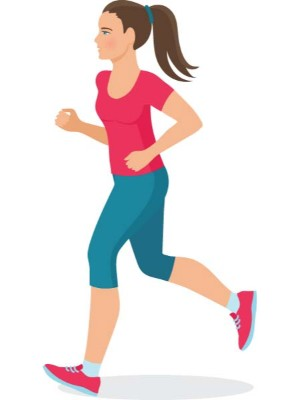
\includegraphics[width=0.29\columnwidth]{figures/I30.jpg}} & {
\includegraphics[width=0.3\columnwidth]{figures/I29.jpg}} & {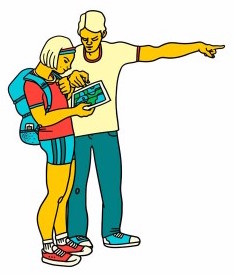
\includegraphics[width=0.3\columnwidth]{figures/I28.jpg}} \\
\hline
What is the woman doing? & What is the woman doing? & What is the man doing? \\
\hline
\end{tabular}
\caption{\label{tab:test-sample-items} The annotation test set items with their targeted questions. In the untargeted form, the question for each is \textit{What is happening?} From left to right, the examples represent one intransitive, transitive and ditransitive item.}
\end{center}
\end{table}

The test set parallels the development set and consists of one intransitive, one transitive and one ditransitive item; it is shown in Table~\ref{tab:test-sample-items}. Agreement and Cohen's kappa scores are given in Table~\ref{tab:agreement}, broken down by different criteria.  The following sections will examine the results, comparing verbs types (transitivity), targeted and untargeted items, the five features, and NS and NNS participants.

%\md{We had the horizontal space, so I spelled all the features out - is it too much?}
\begin{table*}[htb!]
\begin{center}
\begin{tabular}{|l|l|l|l|l||l|l||l|}
\hline
Set	& Total	& A1Yes & A2Yes & AvgYes & Chance & Agree & Kappa \\
\hline
\hline
Intransitive & 2155 & 0.863 & 0.855 & 0.859 & 0.758 & 0.978 & 0.910 \\
\hline
Transitive & 2155 & 0.780 & 0.774 & 0.777 & 0.653 & 0.949 & 0.853 \\
\hline
Ditransitive & 2155 & 0.812 & 0.786 & 0.799 & 0.678 & 0.924 & 0.764 \\ 
\hline
\hline
Targeted & 3390 & 0.829 & 0.818 & 0.824 & 0.709 & 0.949 & 0.823 \\
\hline
Untargeted & 3075 & 0.806 & 0.790 & 0.798 & 0.678 & 0.952 & 0.872 \\
\hline
\hline
Core Event & 1293 & 0.733 & 0.717 & 0.725 & 0.601 & 0.923 & 0.808 \\
\hline
Verifiability & 1293 & 0.845 & 0.817 & 0.831 & 0.719 & 0.968 & 0.884 \\
\hline
Answerhood & 1293 & 0.834 & 0.831 & 0.833 & 0.721 & 0.982 & 0.936 \\
\hline
Interpretability & 1293 & 0.818 & 0.787 & 0.802 & 0.682 & 0.919 & 0.744 \\
\hline
Grammaticality & 1293 & 0.861 & 0.872 & 0.866 & 0.768 & 0.960 & 0.827 \\
\hline
\end{tabular}
\caption{\label{tab:agreement} Agreement scores broken down by different properties of the test set: total annotations (\textit{Total}), \textit{yes} annotations for Annotator 1 and 2 (\textit{A1Yes}, \textit{A2Yes}), average \textit{yes} annotations (\textit{AvgYes}), total expected chance agreement for \textit{yes}es and \textit{no}s (\textit{Chance}), actual raw agreement (\textit{Agree}) and Cohen's kappa (\textit{Kappa}).}
\end{center}
\end{table*}

\subsection{Transitivity} 
\label{sec:transitivity}
Comparing the intransitive, transitive and ditransitive items reveals an association between agreement and item complexity. The highest raw agreement and Cohen's kappa scores are found with the intransitive item ($97.8\%$, $\kappa=0.910$) and the lowest with the ditransitive ($92.4\%$, $\kappa=0.764$). 

This is as expected, as ditransitive sentences are longer and have more verbal arguments, making for more opportunities for responses to vary (see Table~\ref{tab:ttr}), and thus more opportunities for annotators to disagree on a response. This trend also matches annotator feedback: in a follow-up questionnaire, both noted the ditransitive item as the most difficult to annotate overall, and the intransitive as the easiest.

\subsection{Targeting} 
\label{sec:prompts}
Grouping the annotations into targeted and untargeted sets, the raw agreement scores are comparable ($94.9\%$ vs. $95.2\%$). However, despite a greater degree of response variation, the untargeted group has a higher kappa score ($0.872$ vs. $0.823$).
%
%\md{Still thinking through the connection with AvgYes scores ...}
%
When asked to compare the annotation process for targeted and untargeted items, A2 noted that targeted responses require more concentration and closer consultation of the guidelines. For example, \feat{answerhood} does not allow for targeted responses to modify the subject provided in the question in any way, whereas in answering \textit{What is happening?}, the respondent is free to speak of characters in the pictures in many different ways.  Both A1 and A2 thus describe the annotation of untargeted items as less restrictive and less time-consuming.

\subsection{Features} 
\label{sec:features}
Grouped by feature, the annotations all show raw agreement scores above 91\% and Cohen's kappa scores above 0.74 (Table~\ref{tab:agreement}). For future use of this corpus in content assessment, these kappa scores are comfortably above the 0.67 suggested as a threshhold for meaningful, reliable agreement \citep{landis1977measurement, artstein:massimo:2008}.  I discuss each feature in turn here, highlighting difficulties in coming to an agreement, as such disagreements illustrate some of the impactful ways in which responses vary.

\paragraph{Core event} Isolating whether the main content of the picture is being described or not, the \feat{core event} feature is the most relevant of the five for content assessment. All five features are skewed toward \textit{yes} annotations, but with an average \textit{yes} rate of 72.5\%, core event is the least skewed; i.e., more responses receive a \textit{no} annotation for \feat{core event} than for any other feature.

\feat{Core event} has the second lowest inter-annotator agreement kappa score, at 0.808. This is somewhat lower than expected, as the pre-adjudication development set score was 0.889. This appears to be largely attributable to the difficulty of the ditransitive item, challenging for both participants and annotators (section~\ref{sec:transitivity}). 

The main issue in this case has to do with the amount of specificity required to be the core event.  The development set item depicts a man delivering a package to a woman, and most responses describe this as such a transaction, using \textit{give}, \textit{deliver} or \textit{receive}. The test set item shows a man giving directions to a woman (Table~\ref{tab:test-sample-items}), and this resulted in a greater degree of variation. Many  (particularly NNS) responses portray this not as a canonical \textit{giving directions} event but as \textit{pointing}, 
%\textit{guiding}, 
\textit{helping a lost person} or \textit{reading a map}, with A2 more likely to accept these less specific descriptions.

Similarly, but to a lesser extent, the transitive item, which shows a woman hugging a dog (Table~\ref{tab:test-sample-items}), resulted in disagreements where A2 accepts the word \textit{pet} as the object, but A1 rejects such responses as too vague. Despite the acceptable scores for \feat{core event} agreement, the fact that many disagreements hinge on particular word choice or annotators having minor differences in interpretation of the event suggest that greater agreement could be achieved by providing annotators with suggestions about the acceptable content for each response. In other words: by more clearly determining the desired level of specificity of a response---for the verb or its arguments---agreement could be higher. The desired specificity may vary in accordance with the intended use of the annotations; in the current annotations, the standard discussed between annotators and in the guidelines included pragmatic considerations like naturalness, native-likeness and effort.
% \md{Would determining the appropriate level of specificity require knowing the end use of the annotation?}
% \lk{I tried to address it. What do you think now?}
% \md{Nice work!}

\paragraph{Verifiability} On the flipside of the question of whether the core semantic content is expressed is the question of whether any extraneous content is added, or any content used in a way which cannot be verified from the picture.  The average \textit{yes} rate for \feat{verifiability} is 83.1\%, making it the third most skewed feature.

The raw agreement score is 96.8\%, and the kappa score is 0.884. By both measures, this is the second highest agreement score, after \feat{answerhood}. Of 42 disagreements for \feat{verifiability}, annotators agree that at least eight are avoidable. Of these, five involve the incorrect use of plurals. For example, A1 accepted \textit{A man is pointing the way for the women}, when the image shows only one woman, but the guidelines reject such responses. Two other errors stem from inaccuracy, with respondents referring to a dog in the illustration as a cat. Each annotator incorrectly accepted one such response. One disagreement involved the misspelling of a crucial object: \textit{The woman is holding the pat}. It is unclear whether \textit{pet} or \textit{cat} was intended. This should render the response unverifiable, but A1 accepted it.

The remaining disagreements are attributable to different opinions about inferences, with A2 being, in general, more strict.  For the ditransitive item, for example, both annotators accept responses that refer to the woman as a \textit{hiker}, but only A1 accepts responses where the man and woman are collectively referred to as hikers. For the intransitive item depicting a woman running, A1 accepts multiple responses that refer to this as \textit{a race}, as well as responses that infer the runner's motivation (fitness, leisure, etc.). I believe such differences are unavoidable in this annotation task. Adding more detail to the guidelines might help reduce disagreements about inferences, but the guidelines are nearly 40 pages and expanding them to cover various contingencies would certainly add to annotator demand and fatigue.
%The rate of such disagreements might be reduced slightly by adding more detail to the annotation guidelines or having annotators calibrate their ratings with an extended set of sample items, but these increased demands on annotators might also lead to greater annotator fatigue. In other words, the current definition of the feature is a compromise.

\paragraph{Answerhood} Capturing the semantic content of the picture isn't the only criterion for determining the quality of a response; the \feat{answerhood} feature was added largely as a way to identify responses that simply do not follow the instructions. Such responses tend to fall into one of the following categories:

\begin{enumerate}
\item Responses that do not directly answer the given question, perhaps by reframing the perspective so that it seems like a different question was asked, e.g., \textit{He may get fat eating pizza}, in response to \textit{What is the boy doing?} (Table~\ref{tab:dev-transitive});
\item Responses that are gibberish or very low-effort and entered only so the participant can proceed to the next item, e.g., \textit{Hey man};
\item ``Troll'' responses that attempt to be clever or obscene at the cost of attempting a direct answer, e.g., \textit{How is the pizza staying perfectly horizontal when the boy is holding it so close to the tip?}, in response to \textit{What is happening?} (Table~\ref{tab:dev-transitive}).
\end{enumerate}

The majority of participants do attempt to follow the instructions and answer the question, however, and it is unsurprising that this feature skews strongly toward \textit{yes} annotations and results in the highest raw agreement (98.2\%) and kappa (0.936) scores among the five features.

Of 23 disagreements, seven stem from one annotator failing to enforce the requirement that a targeted response subject be either an appropriate pronoun or the exact subject given in the question, without adjectives, relative clauses or other modifiers. Given the question \textit{What is \textbf{the woman} doing?}, for example, the responses \textit{The \textbf{lady} is running} and \textit{The woman \textbf{who in pink} is running} were incorrectly accepted by one annotator each.  While this criterion may seem strict, this subject-identity rule separates the task of identifying an attempt to answer the question from the task of verifying information (see \feat{verifiability} above).

Another ten disagreements involve responses lacking a progressive verb, generally required as an indication that the response refers to the specific action in the image and does not merely describe a state or a general truth (cf., e.g., \textit{The woman is running} vs. \textit{The woman runs}). Annotator fatigue thus appears to account for the majority of \feat{answerhood} disagreements.
%\smallskip

\paragraph{Interpretability} The average \textit{yes} rate for \feat{interpretability} is 0.802; only \feat{core event} is less skewed: responses were thus also more likely to be unacceptable.
%
The raw agreement score is 91.9\% and kappa is 0.744, the lowest scores among the five features. This was anticipated, because \feat{interpretability} is perhaps the most difficult to define, leaving room for annotators' personal judgments. Annotators must decide whether a given response evokes a clear mental image, regardless of how well that mental image matches the PDT image.  In this way, responses such as \textit{The man is working} which may %contain all \feat{core event} information and 
be completely \feat{verifiable} may still fall short, in that the man could be picking fruit, building a bridge, and so forth.

The guidelines place some restrictions on what it means to be a clear mental image. To begin with, if one were to illustrate the response, the result would be a complete, representational, canonical image. It would not be necessary to guess at major elements, like subjects or objects. 
%
All necessary semantic arguments would be identifiable from the sentence and thus not obscured or out of the frame in the mental image.
%
Vague language should be avoided, but human gender does not need to be specified, especially when a non-gendered word like \textit{doctor} or \textit{teacher} is natural. 

Consider a response like \textit{A woman is receiving a package}.  By these criteria, the response is annotated as 0 because the person or entity delivering the package is not specified, and an illustrator would need to either guess or compose the image with the deliverer conspicuously out of the frame. \textit{A man is delivering a package}, on the other hand, would be accepted. An illustrator could simply show a delivery person carrying a package, as an indirect object is not necessary for the verb \textit{deliver}.

Among the 105 annotator disagreements, fatigue accounts for roughly 30; this is difficult to determine precisely because annotators expressed difficulty in identifying a single root cause for many disagreements. Those that are clearly attributable to annotator error tend to involve responses with some internal inconsistency, as with subject-verb disagreements, where the number of the subject is uninterpretable. Among true disagreements, the level of specificity is often the point of contention, as with \feat{core event}. For example, A1 accepted several transitive item responses with the verb \textit{love}, as in \textit{The woman loves her dog} (Table~\ref{tab:test-sample-items}). A2 argued that these are too vague to illustrate as an action, but A1 disagreed. This disagreement may also hinge on differing judgments regarding the use of \textit{love} as a dynamic verb, and such idiolectal differences are an unavoidable source of noise in annotation work (citation?)\lk{citation?}. As mentioned above (see \feat{Verifiability}), expanding the guidelines might help cover some such situations, but likely at the cost of increased annotator fatigue.

\paragraph{Grammaticality} The \feat{grammaticality} feature is the most heavily skewed one, with an average \textit{yes} rate of 86.6\%.  As the only non-semantic annotation, this is perhaps not surprising.

Grammaticality has a raw agreement score of 96.0\% and a kappa of 0.827. Among 52 disagreements, annotators concurred in discussion that 19 involve an avoidable annotator error. These are primarily responses with typos, misspellings, subject-verb disagreement and bare nouns, all rejected by the annotation rules. Such cases are likely attributable to annotator fatigue.

% http://www.cs.rochester.edu/~tetreaul/acl11-mturk-grammar.pdf
The remainder reflect an unavoidable level of disagreement. Many of these stem from differing interpretations of bare nouns as either errors or as acceptable mass nouns, as in \textit{The man is giving \textbf{direction} to the tourist}. In several cases, annotators disagree over prepositions, which are known to be a common source of disagreement and pose special challenges in the context of learner language \citep{tetreault-chodorow:2008:HJCL,tetreault:chodorow:08}. For example, annotators could not agree on the grammaticality of the prepositions in \textit{The girl is asking for help \textbf{to} the man} and \textit{The girl is hugging \textbf{with} her cat}. 

\subsection{NS \& NNS responses}
\label{NSandNNSagreement}
Response quality and annotation agreement were also calculated separately for NS and NNS responses, as shown in Table~\ref{tab:NSvNNSagreement}. The average rate of \textit{yes} annotations is used here as an indication of response quality. Comparing this \textit{yes} rate shows that the NNSs outperform the NSs by between roughly 8\% and 12\% on all features except \feat{grammaticality}. It is not surprising that NSs outperform NNSs on this feature (90.2\% to 79.3\%), but to account for their superior performance on the other features, one must consider the fact that the NNSs were recruited from ESL courses and performed the task with peers and researchers present. The NNSs were more likely to make a good faith effort than the NSs, the majority of whom performed the task anonymously and remotely. Furthermore, 
%only NSs were asked to provide two responses to each item; 
with twice as many responses to provide for each item for NSs, fatigue and boredom may have been a contributing factor.
%; related task effects and fatigue are also likely contributing factors.

%% LK NTS:
%%intransitive is I30 (woman is running)
%%transitive is I29 (woman is hugging dog)
%%ditransitive is I28 (man is giving directions)
%\begin{table*}[htb!]
%\begin{center}
%\begin{tabular}{|l||l|l||l|l||l|l||l|l||l|l|}
%\hline
% & \multicolumn{2}{|c||}{Total} & \multicolumn{2}{|c||}{AvgYes} & \multicolumn{2}{|c||}{Chance} & \multicolumn{2}{|c||}{Agree} & \multicolumn{2}{|c|}{Kappa} \\
%\hline
% Set & NS & NNS & NS & NNS & NS & NNS & NS & NNS & NS & NNS \\
%\hline
%\hline
%Intrans & 1450 & 705 & 0.814 & 0.952 & 0.697 & 0.909 & 0.974 & 0.987 & 0.914 & 0.859 \\
%\hline
%Trans & 1450 & 705 & 0.768 & 0.796 & 0.643 & 0.675 & 0.949 & 0.949 & 0.857 & 0.843 \\ %%LK: Yes, 0.949 is correct in both cases here
%\hline
%Ditrans & 1450 & 705 & 0.794 & 0.808 & 0.672 & 0.689 & 0.922 & 0.928 & 0.762 & 0.767 \\ 
%\hline
%\hline
%Target & 2340 & 1050 & 0.812 & 0.849 & 0.695 & 0.743 & 0.948 & 0.950 & 0.829 & 0.807 \\
%\hline
%Untarg & 2010 & 1065 & 0.768 & 0.855 & 0.643 & 0.753 & 0.949 & 0.959 & 0.856 & 0.833 \\
%\hline
%\hline
%Core & 870 & 423 & 0.686 & 0.805 & 0.569 & 0.686 & 0.922 & 0.927 & 0.819 & 0.767 \\
%\hline
%Verif & 870 & 423 & 0.807 & 0.882 & 0.688 & 0.791 & 0.970 & 0.962 & 0.904 & 0.819 \\
%\hline
%Answer & 870 & 423 & 0.800 & 0.899 & 0.680 & 0.819 & 0.977 & 0.993 & 0.928 & 0.961 \\
%\hline
%Interp & 870 & 423 & 0.764 & 0.881 & 0.638 & 0.789 & 0.910 & 0.936 & 0.752 & 0.697 \\
%\hline
%Gramm & 870 & 423 & 0.902 & 0.793 & 0.823 & 0.671 & 0.962 & 0.955 & 0.786 & 0.863 \\
%\hline
%\end{tabular}
%\caption{\label{tab:NSvNNSagreement} Comparing agreement for NS and NNS responses, with agreement scores broken down by different properties of the test set: total annotations (\textit{Total}), average \textit{yes} annotations (\textit{AvgYes}), total expected chance agreement for \textit{yes}es and \textit{no}s (\textit{Chance}), actual raw agreement (\textit{Agree}) and Cohen's kappa (\textit{Kappa}).}
%\end{center}
%\end{table*}
\begin{table}[htb!]
\begin{center}
\begin{tabular}{|l||l|l||l|l|}
\hline
 & \multicolumn{2}{|c||}{AvgYes} & \multicolumn{2}{|c|}{Kappa} \\
\hline
 Set & NS & NNS & NS & NNS \\
\hline
\hline
%Intrans  & 0.814 & 0.952 & 0.914 & 0.859 \\
%\hline
%Trans  & 0.768 & 0.796 & 0.857 & 0.843 \\ %%LK: Yes, 0.949 is correct in both cases here
%\hline
%Ditrans  & 0.794 & 0.808 & 0.762 & 0.767 \\ 
%\hline
%\hline
%Target  & 0.812 & 0.849 & 0.829 & 0.807 \\
%\hline
%Untarg  & 0.768 & 0.855 & 0.856 & 0.833 \\
%\hline
%\hline
Core  & 0.686 & 0.805 & 0.819 & 0.767 \\
\hline
Verif  & 0.807 & 0.882 & 0.904 & 0.819 \\
\hline
Answer  & 0.800 & 0.899 & 0.928 & 0.961 \\
\hline
Interp  & 0.764 & 0.881 & 0.752 & 0.697 \\
\hline
Gramm  & 0.902 & 0.793 & 0.786 & 0.863 \\
\hline
\end{tabular}
\caption{\label{tab:NSvNNSagreement} NS and NNS test set responses: average \textit{yes} annotations (\textit{AvgYes}) and Cohen's kappa (\textit{Kappa}).}
\end{center}
\end{table}


Turning to the question of annotation quality, raw agreement scores are high among both groups, ranging from 91\% to 99.3\% (not shown)\lk{add raw agreement?}. Notably, for \feat{core event}, \feat{verifiability} and \feat{interpretability}, kappa scores are higher for NS responses than for NNS ones; i.e., annotators agree more on NS responses for these features. It may be no coincidence that these three features are the most closely tied to meaning, while \feat{answerhood} gets at pragmatics and \feat{grammaticality} focuses on form correctness.

The lower kappa score for NS \feat{answerhood} is also attributable to task effects, as a second response (as required of NSs) is more likely to be off topic or in bad faith. For \feat{grammaticality}, kappas for annotator agreement are higher for NNS responses. A relatively low rate of expected (chance) agreement contributes to this fact. Additionally, annotators note that many grammar problems with NNS responses are obvious (e.g., \textit{The \textbf{man who in yellow} is showing the way to a girl}, see Table~\ref{tab:test-sample-items}), but the few grammar problems in NS data are mostly typos and more easily overlooked due to fatigue (e.g., \textit{The man is giving \textbf{ditections}}).


\section{Annotation Conclusions}\lk{Possibly shorten here and move to Conclusions chapter}
%\lk{Not sure what to call this section}
%\md{It's solid - "Conclusion" strikes me as a little better than "Conclusions", though.}

%\subsection{Annotator feedback}
The SAILS corpus presented here was developed with specific research in mind, but also in the hopes that it may be used to address a broad range of questions. I have demonstrated here a set of binary features that were successfully implemented with reliable levels of inter-annotator agreement. These features were defined with an eye toward content analysis and ICALL, but I believe the annotations and raw responses could find uses in question answering, dialog systems, pragmatic modeling, visual references and other challenges in natural language processing. The feature set could also be expanded to better suit other purposes, and the task could easily be extended to include new items. It could also be improved by adding participants from a wider variety of L1s. Guidelines, task materials and annotation tools are included with the corpus.\footnote{https://github.com/sailscorpus/sails}
%\footnote{A non-anonymous github link will be included here in the final version.}

%\smallskip
A number of lessons have been learned in this process, and as I intend this work to be extendable, a few suggestions are in order. The inclusion of any symbols or numerals in items should be avoided as they resulted in response complications; some participants gave clever ``meta'' responses (\textit{She's breathing in music notes}, rather than \textit{She's singing}), and others focused on the symbols rather than the abstract concepts they represent (\textit{The teacher is teaching `2 $+$ 2 $=$ 4'}, rather than \textit{The teacher is teaching math}). The comparison of crowdsourced NS data with the data of known NS participants and the NNS student data makes it clear that motivations and task environment can affect the quality of responses.
%, and these factors must be considered during data collection.

%\smallskip
%The current work is appropriate for a broad examination of variation; if one has more specific research questions in mind, however, a more tailored approach to this kind of data collection and annotation would likely mean more efficiency in terms of effort and expense. 
Additionally, more clearly defining acceptable \feat{core events} could lessen the ambiguity for annotators. While I intend the NS responses collected here to be useful for comparing with NNS responses and addressing related research questions, for specific applications like language testing, the use of expert annotators and constructed reference materials or gold standards may be more appropriate or cost effective \citep{somasundaran:chodorow:14}.
